\documentclass[border=2pt]{standalone}
\usepackage{pgfplots}
\pgfplotsset{compat=1.16}
\begin{document}
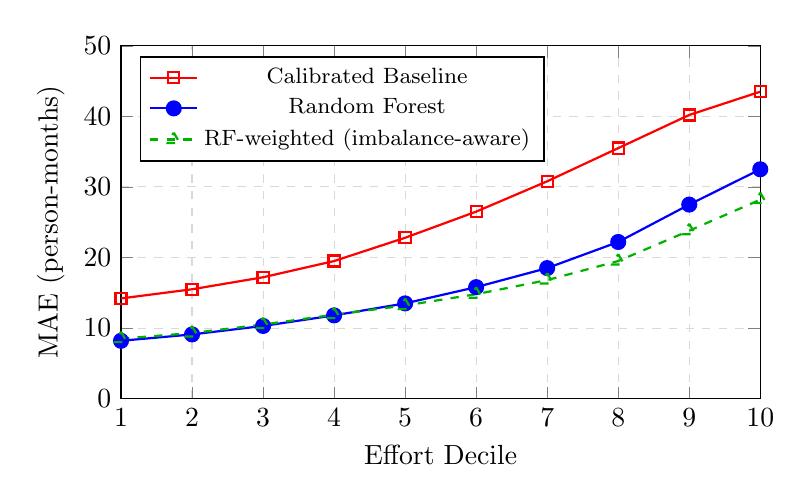
\begin{tikzpicture}
\begin{axis}[
    width=0.8\linewidth,
    height=0.5\linewidth,
    xlabel={Effort Decile},
    ylabel={MAE (person-months)},
    xmin=1, xmax=10,
    ymin=0, ymax=50,
    xtick={1,2,3,4,5,6,7,8,9,10},
    ytick={0,10,20,30,40,50},
    legend pos=north west,
    grid=major,
    grid style={dashed,gray!30},
    legend style={font=\footnotesize}
]
\addplot[color=red, mark=square, thick, mark size=2pt] coordinates {
    (1,14.2) (2,15.5) (3,17.2) (4,19.5) (5,22.8) (6,26.5) (7,30.8) (8,35.5) (9,40.2) (10,43.5)
};
\addlegendentry{Calibrated Baseline}
\addplot[color=blue, mark=*, thick, mark size=2.5pt] coordinates {
    (1,8.2) (2,9.1) (3,10.3) (4,11.8) (5,13.5) (6,15.8) (7,18.5) (8,22.2) (9,27.5) (10,32.5)
};
\addlegendentry{Random Forest}
\addplot[color=green!70!black, mark=triangle, thick, dashed, mark size=2.5pt] coordinates {
    (1,8.5) (2,9.3) (3,10.5) (4,11.9) (5,13.2) (6,14.8) (7,16.8) (8,19.5) (9,23.8) (10,28.2)
};
\addlegendentry{RF-weighted (imbalance-aware)}
\end{axis}
\end{tikzpicture}
\end{document}
